\documentclass[12pt,a4paper]{article}
\usepackage{cmap} % Makes the PDF copiable. See http://tex.stackexchange.com/a/64198/25761
\usepackage[T1]{fontenc}
\usepackage[brazil]{babel}
\usepackage[utf8]{inputenc}
\usepackage{amsmath}
\usepackage{amsfonts}
\usepackage{amssymb}
\usepackage{amsthm}
\usepackage{textcomp} % \degree
\usepackage{gensymb} % \degree
\usepackage[usenames,svgnames,dvipsnames]{xcolor}
\usepackage{hyperref}
\usepackage{multicol}
\usepackage{graphicx}
\usepackage[margin=2cm]{geometry}
\usepackage{systeme}

\hypersetup{
    colorlinks = true,
    allcolors = {blue}
}

% TODO: Consider using exsheets
% http://linorg.usp.br/CTAN/macros/latex/contrib/exsheets/exsheets_en.pdf
%
% http://ctan.org/tex-archive/macros/latex/contrib/exercise/
% Options: answerdelayed,lastexercise,noanswer
\usepackage[answerdelayed,lastexercise]{exercise}

\addto\captionsbrazil{%
\def\listexercisename{Lista de exerc\'icios}%
\def\ExerciseName{Exerc\'icio}%
\def\AnswerName{Solu\c{c}\~ao do exerc\'icio}%
\def\ExerciseListName{Ex.}%
\def\AnswerListName{Solu\c{c}\~ao}%
\def\ExePartName{Parte}%
\def\ArticleOf{de\ }%
}

\renewcommand{\ExerciseHeaderTitle}{(\ExerciseTitle)\ }
\renewcommand{\ExerciseListHeader}{%\ExerciseHeaderDifficulty%
\textbf{%\ExerciseListName\
\ExerciseHeaderNB.\ %
%\ --- \
\ExerciseHeaderTitle}%
%\ExerciseHeaderOrigin
\ignorespaces}
\renewcommand{\AnswerListHeader}{\textbf{\ExerciseHeaderNB.\ (\AnswerListName)\ }}

\newcommand*\ger[1]{\operatorname{ger}\left\{#1\right\}}
\newcommand*\R{\mathbb{R}}

% Loop Space / CC BY-SA-3.0 / https://tex.stackexchange.com/a/2238/25761
\newenvironment{amatrix}[1]{%
  \left[\begin{array}{@{}*{#1}{c}|c@{}}
}{%
  \end{array}\right]
}

% Loop Space / CC BY-SA-3.0 / https://tex.stackexchange.com/a/3164/25761
%--------grstep
% For denoting a Gauss' reduction step.
% Use as: \grstep{\rho_1+\rho_3} or \grstep[2\rho_5 \\ 3\rho_6]{\rho_1+\rho_3}
\newcommand{\grstep}[2][\relax]{%
   \ensuremath{\mathrel{
       {\mathop{\longrightarrow}\limits^{#2\mathstrut}_{
                                     \begin{subarray}{l} #1 \end{subarray}}}}}}

\renewcommand{\theenumi}{\alph{enumi}}
\renewcommand\labelenumi{(\theenumi) }

\newcommand*\tipo{Prova II}
\newcommand*\turma{PRO112-02U}
\newcommand*\disciplina{ALI0001}
\newcommand*\eu{Helder G. G. de Lima}
\newcommand*\data{04/10/2017}

\author{\eu}
\title{\tipo - \disciplina}
\date{\data}

\begin{document}
\thispagestyle{empty}
\newgeometry{margin=2cm,bottom=0.5cm}
\begin{center}

\includegraphics[width=9.0cm]{marca} \\
\textbf{\tipo\ (\disciplina / \turma)} \\
Prof. \eu\footnote{
Este é um material de acesso livre distribuído sob os termos da licença \href{https://creativecommons.org/licenses/by-sa/4.0/deed.pt_BR}{Creative Commons Atribuição-CompartilhaIgual 4.0 Internacional}}
\end{center}

\noindent Nome do(a) aluno(a): \underline{\hspace{9,7cm}} Data: \underline{\data}

%\section*{Instruções}
\begin{center}\fbox{
\begin{minipage}{14cm}

{\footnotesize
\begin{itemize}
\renewcommand{\theenumi}{\Roman{enumi}}
\item Identifique-se em todas as folhas.
\item Mantenha o celular e os demais equipamentos eletrônicos desligados durante a prova.
\item Resolva (integralmente) apenas as questões de que precisar para somar 10,0 pontos.
\end{itemize}
}

\end{minipage}
}
\end{center}

\section*{Questões}
\begin{ExerciseList}
\Exercise[title={2,5}]
Seja $V = \{ (x, y) \in \R^2 \mid y >0 \}$.
\begin{enumerate}
\item O conjunto $V$ é um subespaço de $\R^2$ com as operações usuais de adição e de multiplicação por escalar? Justifique algebricamente e represente geometricamente.
\item Suponha que sejam definidas em $V$ uma ``adição'' e uma ``multiplicação por escalar'' tais que, para quaisquer $v = (x_1, y_1) \in V$, $w = (x_2, y_2) \in V$ e $k \in \R$, tenhamos:
\[
\begin{cases}
    v + w = (x_1, y_1) + (x_2, y_2) = (x_1 + x_2+1, y_1 y_2),\\
k \cdot v = k \cdot (x_1, y_1) = (kx_1+k-1, {y_1}^k).
\end{cases}
\]
Sabendo que $V$, com essas novas operações de $+$ e $\cdot$, é um espaço vetorial, encontre e represente geometricamente:
\begin{enumerate}
\item O elemento $\vec{0}$ de $V$, ou seja, aquele que faz o papel de vetor nulo deste espaço vetorial.
\item O vetor $w = -v$ que é o oposto de $v = (x,y)$ em relação a adição.
\item Dois vetores $u$ e $v$ de $V$ (escolha valores \textit{numéricos}), bem como os resultados das operações $u+v$, $2v$ e $-v$.
\end{enumerate}
\end{enumerate}
\Answer
\begin{enumerate}
\item O conjunto $V$ não é um subespaço de $\R^2$ com as operações usuais pois não é fechado em relação à multiplicação por escalar. Por exemplo, se $k = -1 \in \R$ e $w = (x,y) \in V$ então $k \cdot w = (kx,ky)$ e como $y>0$, tem-se $ky<0$ e $k \cdot w \not\in V$.
\begin{center}
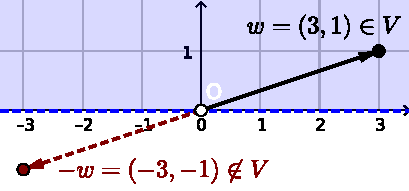
\includegraphics[width=8cm]{img/prova-2-pro-1a-exemplo-negativo}
\end{center}
\item
\begin{enumerate}
\item Se $\vec{0} = (a,b)$ é o vetor nulo, então para todo $w = (x,y) \in V$ deve ocorrer $\vec{0}+w = w$, ou seja, $(a,b)+(x,y) = (x,y)$. Usando a definição da operação $+$, isso equivale a $(a + x + 1, b y) = (x, y)$, isto é, $a+x+1 = x$ e $by = y$. Assim, $a = -1$, $b = 1$ e $\vec{0} = (-1,1)$.
\item Dado $v = (x,y)$, o seu oposto $w = (c,d)$ deve satisfazer $v+w = \vec{0}$, isto é, $(x,y) + (c,d) = (x+c+1, yd) = (-1,1)$, o que equivale a $x+c+1=-1$ e $yd = 1$. Assim, $c=-x-2$ e $d = 1/y$, ou seja, $w = -v = (-x-2, 1/y)$.
\item Considerando $u = (-3,2)$ e $v = (1,2)$, tem-se $u+v = (-1, 4)$, $2v = (3,4)$ e $-v = (-3,1/2)$, como na figura a seguir:
\begin{center}
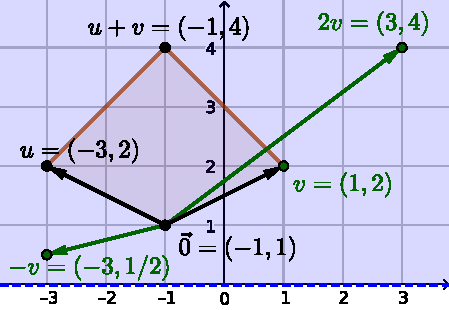
\includegraphics[width=10cm]{img/prova-2-pro-1bc-exemplo-ops}
\end{center}
\end{enumerate}
\end{enumerate}

\Exercise[title={2,5}] Mostre que as matrizes simétricas de ordem $2 \times 2$ formam um subespaço vetorial do espaço de todas das matrizes $2 \times 2$. Obtenha uma base e a dimensão deste subespaço. Justifique.
\Answer Seja $S$ o conjunto das matrizes simétricas de ordem $2 \times 2$. Para que $S$ seja um subespaço, a soma de vetores de $S$ deve ser um vetor de $S$, e o resultado da multiplicação de um vetor de $S$ por qualquer escalar também deve ser um vetor de $S$. Considere $A_1, A_2 \in S$ e $k \in \R$. Então $A_i^T = A_i$ e
\[
(A_1 + A_2)^T
= A_1^T + A_2^T
= A_1 + A_2
\]
\[
  (k A_1)^T
= k (A_1^T)
= k A_1
\]
Portanto, $A_1+A_2 \in S$ e $kA_1 \in S$, ou seja, $S$ é um subespaço vetorial. Se
$A
= \begin{bmatrix}
a & b \\ c & d
\end{bmatrix}
\in S$ então $b=c$, isto é, $A
= \begin{bmatrix}
a & b \\ b & d
\end{bmatrix}
=
a \begin{bmatrix}
1 & 0 \\ 0 & 0
\end{bmatrix}
+b \begin{bmatrix}
0 & 1 \\ 1 & 0
\end{bmatrix}
+d \begin{bmatrix}
0 & 0 \\ 0 & 1
\end{bmatrix}$. Portanto, $S$ é gerado por
\[
B=
\left\{
\begin{bmatrix}
1 & 0 \\ 0 & 0
\end{bmatrix},
\begin{bmatrix}
0 & 1 \\ 1 & 0
\end{bmatrix},
\begin{bmatrix}
0 & 0 \\ 0 & 1
\end{bmatrix}
\right\}.
\]
Os vetores de $B$ são linearmente independentes pois
\[
a \begin{bmatrix}
1 & 0 \\ 0 & 0
\end{bmatrix}
+b \begin{bmatrix}
0 & 1 \\ 1 & 0
\end{bmatrix}
+d \begin{bmatrix}
0 & 0 \\ 0 & 1
\end{bmatrix}
=\begin{bmatrix}
a & b \\ b & d
\end{bmatrix}
=
\begin{bmatrix}
0 & 0 \\ 0 & 0
\end{bmatrix}
\]
só é possível se $a=b=d=0$. Consequentemente, $B$ é uma base de $S$ e $\dim S = 3$.


\Exercise[title={2,5}] Prove ou dê um contraexemplo para as afirmações a seguir, a respeito do espaço $W = \ger{
\begin{bmatrix}
1 & 2 \\ 0 & 2
\end{bmatrix},
\begin{bmatrix}
1 & 0 \\ 2 & 2
\end{bmatrix},
\begin{bmatrix}
1 & 0 \\ 0 & 1
\end{bmatrix},
\begin{bmatrix}
0 & 1 \\ -1 & 0
\end{bmatrix}
}$, justificando todas as suas conclusões:
\begin{enumerate}
\item O espaço $W$ possui algum subespaço de dimensão 2.
\item Toda matriz antissimétrica de ordem $2 \times 2$ pertence a $W$.
\end{enumerate}
\Answer
\begin{enumerate}
\item \textbf{Verdadeiro}: Se $W_1 = \ger{
\begin{bmatrix}
1 & 0 \\ 0 & 1
\end{bmatrix},
\begin{bmatrix}
0 & 1 \\ -1 & 0
\end{bmatrix}
}$ então $\dim W_1 = 2$ pois estes dois vetores são linearmente independentes (não são múltiplos um do outro) e geram $W_1$.
\item \textbf{Verdadeiro}: Se $A =
\begin{bmatrix}
a & b \\ c & d
\end{bmatrix}
$ é antissimétrica, então $a=d=0$ e $c=-b$. Assim,
\[
A =
\begin{bmatrix}
0 & b \\ -b & 0
\end{bmatrix}
=b \begin{bmatrix}
0 & 1 \\ -1 & 0
\end{bmatrix}
\in W,
\]
pois $\begin{bmatrix}
0 & 1 \\ -1 & 0
\end{bmatrix}
\in W$. Portanto, todas as matrizes antissimétricas $2\times 2$ pertencem a $W$.
\end{enumerate}

\Exercise[title={2,5}] Sejam $v_1 = (1,1,0,0)$, $v_2 = (0,1,1,0)$, $v_3 = (0,0,1,1)$ e $v_4 = (1,0,0,1)$ vetores de $\R^4$.
\begin{enumerate}
\item É correto dizer que $\R^4 = \ger{ v_1, v_2, v_3, v_4 }$? Justifique sua conclusão.
\item De quantas maneiras $w = (1,2,3,2)$ pode ser escrito como combinação linear de $v_1, \ldots, v_4$? Por quê?
\end{enumerate}
\Answer
\begin{enumerate}
\item Pode-se averiguar se a afirmação é verdadeira verificando se qualquer $v = (x,y,z,w) \in \R^4$ pode ser escrito como uma combinação linear dos vetores dados, isto é, se existem escalares $k_1, k_2, k_3, k_4 \in \R$ tais que
\[
v = k_1 v_1 + k_2 v_2 +  k_3 v_3 + k_4 v_4
  = k_1 (1,1,0,0)
  + k_2 (0,1,1,0)
  + k_3 (0,0,1,1)
  + k_4 (1,0,0,1).
\]
Isso equivale a verificar a compatibilidade de um sistema linear, como segue:
\[
\systeme[k_1k_2k_3k_4]{
k_1 + k_4 = x,
k_1 + k_2 = y,
k_2 + k_3 = z,
k_3 + k_4 = w
}
\Leftrightarrow
\begin{bmatrix}
1 & 0 & 0 & 1 \\
1 & 1 & 0 & 0 \\
0 & 1 & 1 & 0 \\
0 & 0 & 1 & 1
\end{bmatrix} \cdot
\begin{bmatrix}
k_1\\k_2\\k_3\\k_4
\end{bmatrix}
=
\begin{bmatrix}
x\\y\\z\\w
\end{bmatrix}
\]
Escalonando a matriz ampliada, obtém-se:
\begin{align*}
\begin{bmatrix}
1 & 0 & 0 & 1 & x \\
1 & 1 & 0 & 0 & y \\
0 & 1 & 1 & 0 & z \\
0 & 0 & 1 & 1 & w
\end{bmatrix}
& \rightarrow
\begin{bmatrix}
1 & 0 & 0 & 1 & x \\
0 & 1 & 0 & -1 & y-x \\
0 & 1 & 1 & 0 & z \\
0 & 0 & 1 & 1 & w
\end{bmatrix}
\rightarrow
\begin{bmatrix}
1 & 0 & 0 & 1 & x \\
0 & 1 & 0 & -1 & y-x \\
0 & 0 & 1 & 1 & z-y+x \\
0 & 0 & 1 & 1 & w
\end{bmatrix}\\
& \rightarrow
\begin{bmatrix}
1 & 0 & 0 & 1 & x \\
0 & 1 & 0 & -1 & y-x \\
0 & 0 & 1 & 1 & z-y+x \\
0 & 0 & 0 & 0 & w-z+y-x
\end{bmatrix}
\end{align*}
Assim, o sistema só é possível (e indeterminado) se $w-z+y-x = 0$. Como isso não ocorre para todos os vetores de $\R^4$, conclui-se que $\R^4$ não é gerado pelos vetores dados.

\item Como o vetor $w = (1,2,3,2)$ satisfaz a condição obtida anteriormente, isto é, $2-3+2-1 = 0$, o sistema torna-se possível e indeterminado, o que implica que há infinitas formas de escrevê-lo como combinação linear dos vetores dados.
\end{enumerate}

\Exercise[title={2,5}] Obtenha uma base e a dimensão da interseção $V_1 \cap V_2$, sendo
\[
V_1 = \{ q(x) = ax^2 + bx + c \in P_2 \mid q(1) = 0\}
\quad \text{ e } \quad
V_2 = \{ q(x) = ax^2 + bx + c \in P_2 \mid q(-1) = 0\}.
\]
\Answer Dado $q(x) = ax^2 + bx + c \in V_1 \cap V_2$, tem-se:
\[
\begin{cases}
q(1)  = a + b + c = 0\\
q(-1) = a - b + c = 0
\end{cases}
\Leftrightarrow
\begin{bmatrix}
1 & 1 & 1\\
1 & -1 & 1
\end{bmatrix}
\cdot
\begin{bmatrix}
a \\ b \\ c
\end{bmatrix}
=
\begin{bmatrix}
0 \\ 0
\end{bmatrix}
\]
Escalonando a matriz deste sistema homogêneo, resulta:
\begin{align*}
\begin{bmatrix}
1 & 1 & 1\\
1 & -1 & 1
\end{bmatrix}
\rightarrow
\begin{bmatrix}
1 & 1 & 1\\
0 & -2 & 0
\end{bmatrix}
\rightarrow
\begin{bmatrix}
1 & 1 & 1\\
0 & 1 & 0
\end{bmatrix}
\rightarrow
\begin{bmatrix}
1 & 0 & 1\\
0 & 1 & 0
\end{bmatrix}.
\end{align*}
Assim, $a = -c$ e $b=0$, isto é, $q(x) = -cx^2+c = c(-x^2 + 1) \in \ger{-x^2 + 1}$. Como $\{-x^2 + 1\}$ é linearmente independente, e gera $V_1 \cap V_2$, tal conjunto é uma base de $V_1 \cap V_2$. Logo $\dim{V_1 \cap V_2} = 1$.
\end{ExerciseList}

\begin{center}
BOA PROVA!
\end{center}

%\newpage
%\includegraphics[width=16.384cm]{malha}

\newpage
\restoregeometry
\section*{Respostas}
\shipoutAnswer
\end{document}
